% Atualizado para atender as normas ABNT por Mônica da Silva (04/11/2021)

% --- -----------------------------------------------------------------
% --- Elementos usados na Capa e na Folha de Rosto.
% --- EXPRESSÔES ENTRE <> DEVERÂO SER COMPLETADAS COM A INFORMAÇÂO ESPECÍFICA DO TRABALHO
% --- E OS SÌMBOLOS <> DEVEM SER RETIRADOS 
% --- -----------------------------------------------------------------
\autor{RAFAEL HEITOR CORREIA DE MELO} % deve ser escrito em maiúsculo

\titulo{Uma Proposta de Uso de Dispositivo Háptico
para Treinamento de Anestesia raquidiana}

\instituicao{UNIVERSIDADE FEDERAL FLUMINENSE}

\orientador{Aura Conci, D.Sc.}

%\coorientador{<NOME DO COORIENTADOR>} % se nao existir co-orientador apague essa linha

\local{NITER\'{O}I}

\data{2022} % ano da defesa

\comentario{Tese de Doutorado apresentada ao Programa de P\'{o}s-Gradua\c{c}\~{a}o em Computa\c{c}\~{a}o da \mbox{Universidade} Federal Fluminense como requisito parcial para a obten\c{c}\~{a}o do Grau de \mbox{Doutor em Computa\c{c}\~{a}o}. \'{A}rea de concentra\c{c}\~{a}o: \mbox{Computação Visual.}} %preencha com a sua área de concentração


% --- -----------------------------------------------------------------
% --- Capa. (Capa externa, aquela com as letrinhas douradas)(Obrigatório)
% --- ----------------------------------------------------------------
\capa

% --- -----------------------------------------------------------------
% --- Folha de rosto. (Obrigatório)
% --- ----------------------------------------------------------------
\folhaderosto

% --- -----------------------------------------------------------------
% --- Ficha catalográfica obrigatória na versão final. (Obrigatório)
% --- ----------------------------------------------------------------

\begin{figure}[!ht]
   \centering
   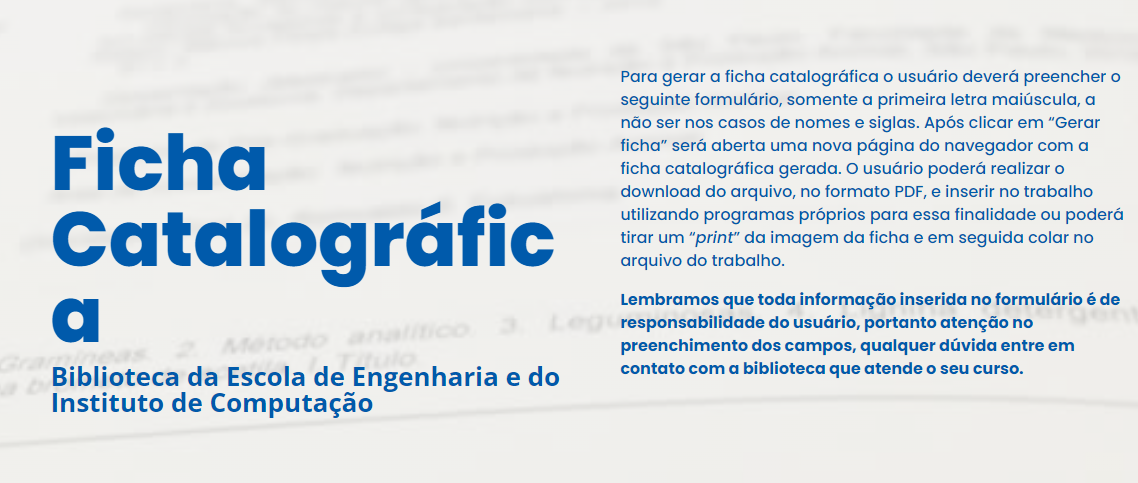
\includegraphics[width=1\linewidth]{capitulos/figuras/ficha_catalografica.png}
   \caption{Local da ficha catalográfica}
\end{figure}

\cleardoublepage


\pagestyle{ruledheader}
\setcounter{page}{1}
\pagenumbering{roman}

% --- -----------------------------------------------------------------
% --- Termo de aprovação. (Obrigatório)
% --- ----------------------------------------------------------------
\cleardoublepage
\thispagestyle{empty}

\vspace{-60mm}

\begin{center}
   {\large RAFAEL HEITOR CORREIA DE MELO}\\
   \vspace{7mm}

   Uma Proposta de uso de Dispositivo Háptico
para Treinamento de Anestesia raquidiana\\
  \vspace{10mm}
\end{center}

\noindent
\begin{flushright}
\begin{minipage}[t]{8cm}

Tese de Doutorado apresentada ao Programa de P\'{o}s-Gradua\c{c}\~{a}o em Computa\c{c}\~{a}o da Universidade Federal Fluminense como requisito parcial para a obten\c{c}\~{a}o do \mbox{Grau} de Doutor em Computa\c{c}\~{a}o. \'{A}rea de concentra\c{c}\~{a}o: \mbox{Computação Visual.} %preencha com a sua área de concentração

\end{minipage}
\end{flushright}
\vspace{1.0 cm}
\noindent
Aprovada em outubro de 2022. \\
\begin{flushright}
 % \parbox{11cm}
  {
  \begin{center}
  BANCA EXAMINADORA \\
  \vspace{6mm}
  \rule{11cm}{.1mm} \\
    Profa. D.Sc. Aura Conci - Orientadora, UFF \\
    \vspace{6mm}
  \rule{11cm}{.1mm} \\
    Prof. D.Sc. Anselmo Cardoso de Paiva, UFMA\\
    \vspace{6mm}
  \rule{11cm}{.1mm} \\
    Prof. D.Sc. Débora Christina Muchaluat Saade, UFF\\
  \vspace{4mm}
  \rule{11cm}{.1mm} \\
    Prof. D.Sc. Fátima de Lourdes dos Santos Nunes Marques, USP\\
    \vspace{6mm}
  \rule{11cm}{.1mm} \\
    Prof. D.Sc. José Viterbo Filho, UFF\\
  \vspace{6mm}
  \end{center}
  }
\end{flushright}
\begin{center}
  \vspace{4mm}
  Niter\'{o}i \\
  %\vspace{6mm}
  2022

\end{center}

% --- -----------------------------------------------------------------
% --- Dedicatoria.(Opcional)
% --- -----------------------------------------------------------------
\cleardoublepage
\thispagestyle{empty}
\vspace*{200mm}

\begin{flushright}
{\em 
    %Dedicatória(s): Elemento opcional onde o autor presta homenagem ou dedica seu trabalho (ABNT, 2005).
    
    Dedico este trabalho a minha esposa, Evelyn, que sempre me apoiou na direção das minhas conquistas e ao meu filho, Rafael, que, ao chegar me apresentou uma nova forma de amar.
}
\end{flushright}
\newpage


% --- -----------------------------------------------------------------
% --- Agradecimentos.(Opcional)
% --- -----------------------------------------------------------------
\pretextualchapter{Agradecimentos}
\hspace{5mm}
%<Elemento opcional, colocado após a dedicatória (ABNT, 2005). >
Agradeço a Deus por me mostrar sempre os caminhos, mesmo nos momentos em que parece que isso não vai acontecer. 

Aos meus pais Julio e Dayse pela preocupação e apoio. Aos meus irmãos Leonardo e Julia pela amizade e companheirismo essenciais nos momentos difíceis.

Agradeço muito a minha orientadora Aura, que mesmo nos momentos de desânimo conseguiu me trazer, em palavras, motivação para seguir em frente.

Ao amigo André que foi essencial em parte dessa caminhada.

À minha família, agradeço a compreensão pelas minhas ausências e minhas desculpas nos momentos de desânimo.



% --- -----------------------------------------------------------------
% --- Resumo em português.(Obrigatório)
% --- -----------------------------------------------------------------
\begin{resumo}

%Elemento obrigatório, constituído de uma sequência de frases concisas e objetivas e não de uma simples enumeração de tópicos, não ultrapassando 500 palavras ABNT NBR 6028:2003.

As anestesias raquidianas são procedimentos cegos que dependem do sentimento do médico no decorrer da inserção da agulha para correta identificação do local de aplicação do líquido anestésico. Em grande parte dos centros de treinamento a primeira experiência tátil do médico em treino tende a ser praticada em pacientes reais. Esta prática, apesar de ser efetuada sob supervisão direta, traz riscos para estes pacientes e possíveis inseguranças aos aprendizes. Técnicas alternativas de uso de \textit{phantoms} e cadáveres no treinamento oferecem uma pequena representatividade em relação às variações de pacientes reais. 
Este trabalho propõe o desenvolvimento de um ambiente virtual para simulação do procedimento que envolve anestesias raquidianas. Considera-se o procedimento de punção com \textit{feedback} tátil e visual usando técnicas de auto treinamento. As sensações táteis do médico em treinamento são simuladas no protótipo através da integração com dispositivo háptico. A geração e visualização dinâmica de modelos de corpos de pacientes baseados em altura e peso também faz parte deste trabalho. Alunos de computação validaram a parte do protótipo que envolve a detecção de diferentes sensações de perfuração de tecidos por meio de experimentos propostos. Finalmente, esta tese  também apresenta um modelo adaptável de um corpo de gestante que possui modelagem de todas as camadas desde a pele das costas até os ossos da coluna vertebral. Modelamos de forma dinâmica as camadas de tecido mais variáveis para permitir uma maior variabilidade de cenários de treinamento. 

{\hspace{-8mm} \bf{Palavras-chave}}: Dispositivo háptico, Treinamento médico, Anestesia raquidiana, Realidade virtual, Ambiente virtual, Paciente virtual Simulação, Retorno tátil.

\end{resumo}

% --- -----------------------------------------------------------------
% --- Resumo em língua estrangeira.(Obrigatório)
% --- -----------------------------------------------------------------
\begin{abstract}

%Elemento obrigatório, em língua estrangeira, com as mesmas características do resumo em língua vernácula (ABNT, 2005).

Spinal anesthesia is a blind procedure where physicians and anesthetists rely on manual feedback to guide their movements through needle insertion. The aim is to identify drug administration locations correctly. For many training centers, the first tactile experience of anesthetists in training occurs in an actual patient under direct supervision. Besides this supervision, there are risks associated with this approach for patients and apprentices. Using phantoms and dead bodies for training offers a low range of scenarios. This work proposes a training environment to simulate spinal anesthesia procedures. The puncture procedure is considered with tactile and visual feedback using self-training techniques. Tactile sensations of the physician in training are simulated in the prototype through integration with a haptic device. The dynamic generation and visualization of patient body models based on height and weight is also part of this work. Computer science students validated the detection of different sensations of tissue perforation related to the procedure through experiments. Finally, this thesis also presents an adaptable model of a pregnant woman's body that models all layers from the skin of the back to the bones of the spine.  We model the most variable tissue layers dynamically to allow more significant training scenarios. 



% O resumo deve ser redigido na terceira pessoa do singular, com verbo na voz ativa, não ultrapassando uma página ou 500 palavras, segundo a ABNT NBR 6028). Evitando-se ouso de parágrafos no meio do resumo, assim como fórmulas, equações e símbolos. Iniciar o resumo situando o trabalho no contexto geral, apresentar os objetivos, descrever a metodologia utilizada, relatar a contribuição própria, comentar os resultados obtidos e finalmente apresentaras conclusões mais importantes do trabalho. 



{\hspace{-8mm} \bf{Keywords}}: Haptics, Medical training, Spinal anesthesia, Virtual reality, Virtual environment, Virtual patient, Simulation, tactile feedback.

\end{abstract}

% --- -----------------------------------------------------------------
% --- Lista de figuras.(Opcional)
% --- -----------------------------------------------------------------
%\cleardoublepage
\listoffigures



% --- -----------------------------------------------------------------
% --- Lista de tabelas.(Opcional)
% --- -----------------------------------------------------------------
\cleardoublepage
%\label{pag:last_page_introduction}
\listoftables
\cleardoublepage

% --- -----------------------------------------------------------------
% --- Lista de abreviatura.(Opcional)
%Elemento opcional, que consiste na relação alfabética das abreviaturas e siglas utilizadas no texto, seguidas das %palavras ou expressões correspondentes grafadas por extenso. Recomenda-se a elaboração de lista própria para cada %tipo (ABNT, 2005).
% --- ----------------------------------------------------------------

\cleardoublepage
\printglossary[type=\acronymtype,title={Lista de Abreviaturas e Siglas}]
\cleardoublepage


% --- -----------------------------------------------------------------
% --- Sumario.(Obrigatório)
% --- -----------------------------------------------------------------

\pagestyle{ruledheader}
\tableofcontents
\pagebreak